% Figure 1: Conceptual Research Framework
\begin{figure}[!htbp]
\centering
\captionsetup{labelfont=it,textfont=normalfont,labelsep=colon,position=above,skip=4pt,singlelinecheck=false,justification=raggedright}
\caption{Research Framework}
\label{fig:framework}
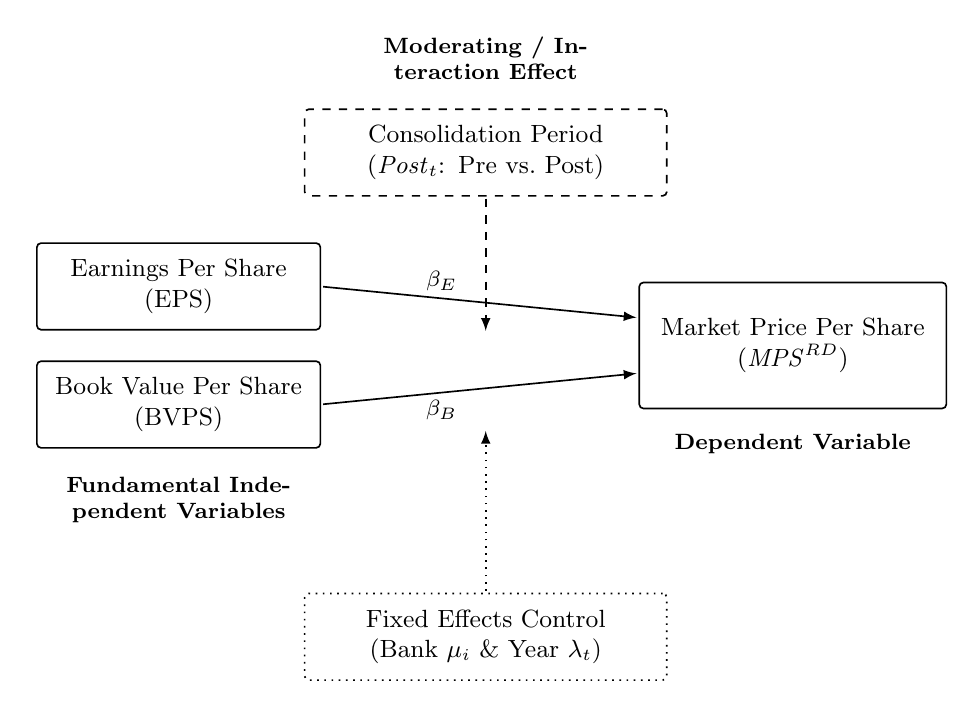
\begin{tikzpicture}[
  every node/.style={font=\small},
  box/.style={rectangle, draw=black, line width=0.6pt, rounded corners=1.5pt, fill=white,
              minimum width=3.60cm, minimum height=1.10cm, text width=3.30cm,
              align=center, inner sep=3pt, outer sep=0pt},
  depbox/.style={rectangle, draw=black, line width=0.6pt, rounded corners=1.5pt, fill=white,
              minimum width=3.90cm, minimum height=1.60cm, text width=3.60cm,
              align=center, inner sep=3pt, outer sep=0pt},
  modbox/.style={rectangle, draw=black, line width=0.6pt, dashed, rounded corners=1.5pt, fill=white,
              minimum width=4.60cm, minimum height=1.10cm, text width=4.30cm,
              align=center, inner sep=3pt, outer sep=0pt},
  ctrlbox/.style={rectangle, draw=black, line width=0.6pt, dotted, rounded corners=1.5pt, fill=white,
              minimum width=4.60cm, minimum height=1.10cm, text width=4.30cm,
              align=center, inner sep=3pt, outer sep=0pt},
  arrow/.style={line width=0.6pt, ->, >=latex, shorten <=1pt, shorten >=1pt},
  modarrow/.style={arrow, dashed},
  ctrlarrow/.style={arrow, dotted},
  edgelabel/.style={font=\footnotesize, fill=white, inner sep=1.5pt},
  heading/.style={font={\footnotesize\bfseries}, align=center}
]

  % Fundamental independent variables
  \node[box] (eps) at (0,1.75) {Earnings Per Share\\(EPS)};
  \node[box] (bvps) at (0,0.25) {Book Value Per Share\\(BVPS)};

  % Dependent variable
  \node[depbox] (mps) at (7.80,1.00) {Market Price Per Share\\($\mathit{MPS}^{RD}$)};

  % Moderator
  \node[modbox] (post) at (3.90,3.45) {Consolidation Period\\($\mathit{Post}_t$: Pre vs.\ Post)};

  % Fixed effects control
  \node[ctrlbox] (fe) at (3.90,-2.70) {Fixed Effects Control\\(Bank $\mu_i$ \& Year $\lambda_t$)};

  % Main effect arrows
  \draw[arrow]
    (eps.east) --
    node[edgelabel, pos=0.38, anchor=south, yshift=1pt] {$\beta_E$}
    ([yshift=10pt]mps.west);

  \draw[arrow]
    (bvps.east) --
    node[edgelabel, pos=0.38, anchor=north, yshift=-1pt] {$\beta_B$}
    ([yshift=-10pt]mps.west);

  % Moderator and fixed-effects arrows
  \draw[modarrow] (post.south) -- (3.90,1.15);
  \draw[ctrlarrow] (fe.north) -- (3.90,-0.05);

  % Figure labels
  \node[heading, anchor=south, text width=4.60cm] at (3.90,4.25)
    {Moderating / Interaction Effect};

  \node[heading, anchor=north, text width=3.60cm] at (0,-0.55)
    {Fundamental Independent Variables};

  \node[heading, anchor=north, text width=3.00cm] at (7.80,0.00)
    {Dependent Variable};

\end{tikzpicture}
\par\vspace{4pt}
{\raggedright\small \textit{Source:} Adapted from \citet{ohlson1995} and \citet{kwon2020}.\par}
\end{figure}
